\chapter{Giovedì 03/04/2020}

\section{Dal modello concettuale al modello logico}
\begin{wrapfigure}{r}{0.35\textwidth}
	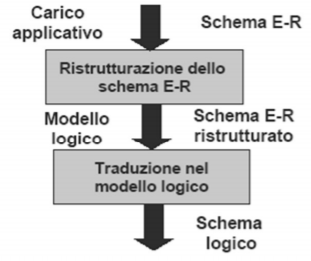
\includegraphics[width=0.9\linewidth]{images/99.PNG} 
	\vspace*{-30pt}
\end{wrapfigure}

\paragraph{Obiettivo} Nel passaggio da modello concettuale a modello logico \emph{traduciamo} in modo automatico lo schema concettuale in uno schema logico che rappresenti gli stessi dati in maniera corretta ed efficiente. Nel compiere questo passaggio indichiamo come dati in ingresso:
\begin{itemize}
	\item lo schema concettuale
	\item il modello logico scelto
	\item le informazioni sul carico applicativo (dimensione dei dati)
\end{itemize}
Otteniamo, in uscita, lo schema logico.
\paragraph{No traduzione immediata} Prima di tradurre dobbiamo ristrutturare lo schema E-R. Obiettivo è:
\begin{itemize}
	\item semplificare (rimuovendo ciò che non può essere rappresentato nel modello logico) 
	\item ottimizzare (tenendo in conto i requisiti di prestazione).
\end{itemize}
\paragraph{Operazioni eseguibili nella ristrutturazione}
\begin{enumerate}
	\item Eliminazione delle generalizzazioni (come già detto vengono perse nel modello logico)
	\item Eliminazione degli attributi multivalore
	\item Analisi ed eventuale eliminazione/aggiunta di ridondanze
	\item Partizionamento/Accorpamento di entità e relationship
\end{enumerate}
\pagebreak
\small
\subsection{Eliminazione delle generalizzazioni}
Le gerarchie devono essere sostituite con entità e relazioni. Scegliamo la soluzione adatta in base al numero e al tipo degli accessi fatti alle singole entità per eseguire le operazioni. 
\begin{itemize}
	\item \textbf{Accorpamento delle figlie della generalizzazione nel genitore}. Questo tipo di sostituzione conviene quando gli accessi al padre e alle figlie sono contestuali.
	Le proprietà delle entità figlie vengono accorpate alle proprietà dell'entità genitore. Aggiungo un ulteriore attributo che mi permette di capire se un'occorrenza del genitore era occorrenza di uno dei figli (o di nessuno con generalizzazioni parziali)
	\begin{figure}[h]
		\begin{subfigure}{0.5\textwidth}
			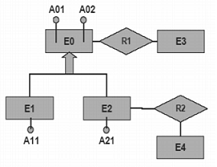
\includegraphics{images/100.PNG} 
			\caption{Schema con generalizzazione}
		\end{subfigure}
		\begin{subfigure}{0.5\textwidth}
			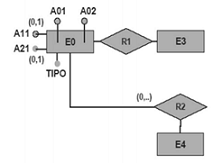
\includegraphics{images/101.PNG}
			\caption{Schema ristrutturato}
		\end{subfigure}
	\end{figure}
	\item \textbf{Accorpamento del genitore della generalizzazione nelle figlie}. Questo tipo di sostituzione conviene con accessi solo alle figlie e questi sono distinti dall'una all'altra. Le entità figlie avranno anche gli attributi dell'entità genitore.
	\begin{figure}[h]
		\begin{subfigure}{0.5\textwidth}
			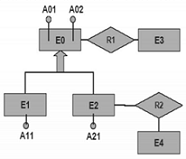
\includegraphics{images/102.PNG} 
			\caption{Schema con generalizzazione}
		\end{subfigure}
		\begin{subfigure}{0.5\textwidth}
			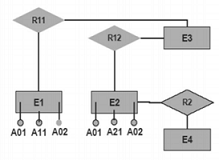
\includegraphics{images/103.PNG}
			\caption{Schema ristrutturato}
		\end{subfigure}
	\end{figure}
	\item \textbf{Sostituzione della generalizzazione con relazioni}. Questo tipo di sostituzione conviene  quando si effettuano accessi separati alle entità figlie e al padre. 
	Non effettuo trasferimenti di attributi, le due nuove entità sono identificate esternamente. In alcuni casi, in base al tipo di generalizzazione, potrei avere bisogno di stabilire dei vincoli di integrità.
	\begin{figure}[h]
		\begin{subfigure}{0.5\textwidth}
			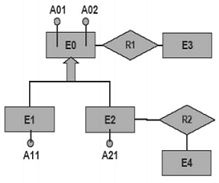
\includegraphics{images/104.PNG} 
			\caption{Schema con generalizzazione}
		\end{subfigure}
		\begin{subfigure}{0.5\textwidth}
			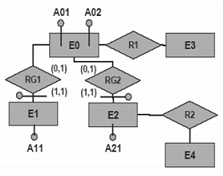
\includegraphics{images/105.PNG}
			\caption{Schema ristrutturato}
		\end{subfigure}
	\end{figure}
\end{itemize}
\pagebreak
\paragraph{Soluzioni ibride} Individuiamo, soprattutto in gerarchie a più livelli, soluzioni ibride. 
\begin{figure}[h]
	\begin{subfigure}{0.5\textwidth}
		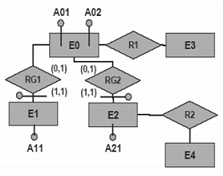
\includegraphics{images/105.PNG} 
		\caption{Schema con generalizzazione}
	\end{subfigure}
	\begin{subfigure}{0.5\textwidth}
		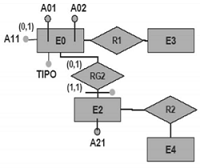
\includegraphics{images/106.PNG}
		\caption{Schema ristrutturato}
	\end{subfigure}
\end{figure}
\normalsize
\subsection{Eliminazione degli attributi multivalore}
\begin{wrapfigure}{r}{0.35\textwidth}
	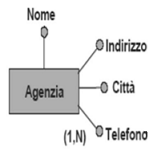
\includegraphics{images/107.PNG} 
	\vspace*{-30pt}
\end{wrapfigure}
\paragraph{Pensiamo a delle soluzioni} Si potrebbe pensare a 
\begin{itemize}
	\item Ripetere le tuple con ogni valore diverso dell'attributo
	\item Una sola tupla dimensionata al numero massimo di numeri di telefono possibili
\end{itemize}
In entrambi i casi si ha spreco di memoria  e con la prima soluzione si potrebbe incorrere in inconsistenze. Segue che la migliore sostituzione consiste nello schema seguente
\begin{center}
	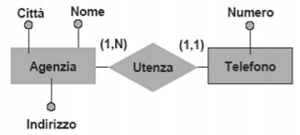
\includegraphics{images/108.PNG}
\end{center}
\subsection{Analisi ed eventuale eliminazione delle ridondanze}
\paragraph{Cos'è una ridondanza} Con ridondanza intendiamo un'informazione significativa, ma derivabile da altre.
\paragraph{Forme di ridondanza in uno schema E-R} 
\begin{itemize}
	\item attributi derivabili da altri attributi della stessa entità (o associazione)
	\begin{center}
		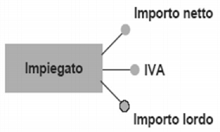
\includegraphics{images/109.PNG}
	\end{center}
	\item attributi derivabili da attributi di altre entità (o associazioni)
	\begin{center}
		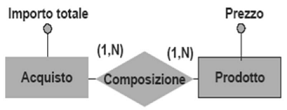
\includegraphics{images/110.PNG}
	\end{center}
	\item associazioni derivabili dalla composizione di altre associazioni (presenza di cicli)
	\begin{center}
		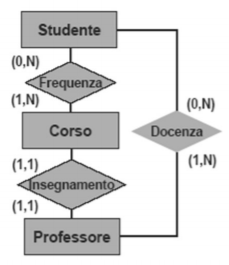
\includegraphics{images/111.PNG}
	\end{center}
\end{itemize}
\subsubsection{Analisi di una ridondanza}
Abbiamo il seguente schema con ridondanza evidente (l'attributo \emph{Numero abitanti}).
\begin{center}
	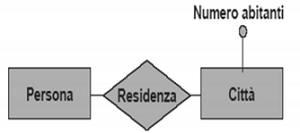
\includegraphics{images/112.PNG}
\end{center}
Devo decidere se eliminare la ridondanza presente o mantenerla in base ad una valutazione del costo delle operazioni
\paragraph{\textcolor{green}{Vantaggi}} Interrogazioni semplificate
\paragraph{\textcolor{red}{Svantaggi}} Appesantimento degli aggiornamenti e maggiore occupazione di spazio
\paragraph{Come analizzo le prestazioni?} Per ottimizzare abbiamo bisogno di analizzare le prestazioni, ma come possiamo fare questo su uno schema concettuale? Prendiamo i seguenti indicatori di prestazione:
\begin{itemize}
	\item spazio: numero di occorrenze previste. Realizziamo una \textbf{tavola dei volumi} in cui elenchiamo i vari elementi e il loro volume (il numero di record).
	\item tempo: numero di occorrenze (di entità e relationship) visitate per portare a termine un'operazione. Partendo dai dati a disposizione costruisco una \textbf{tavola degli accessi} basata su uno schema di navigazione.
\end{itemize}
\subsubsection{Esempio di risoluzione (Mantenere il numeroAbitanti come attributo?)} Riprendiamo lo schema a inizio sessione. Vogliamo eseguire le seguenti operazioni:
\begin{itemize}
	\item \textbf{Operazione 1}: memorizza una nuova persona con la relativa residenza, supponendo che la città sia già presente (500 volte al giorno)
	\item \textbf{Operazione 2}: stampa tutti i dati di una città (incluso il numero di abitanti) (2 volte al giorno)
\end{itemize}
Devo decidere se mantenere l'attributo \emph{numeroAbitanti} o rimuoverlo. La tabella dei volumi è la seguente:
\begin{center}
	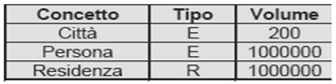
\includegraphics{images/113.PNG}
\end{center}
Analizziamo le tavole degli accessi con e senza ridondanza per entrambe le operazioni
\begin{figure}[h]
	\begin{subfigure}{0.5\textwidth}
		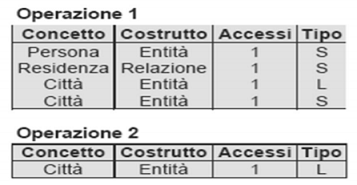
\includegraphics{images/114.PNG} 
		\caption{Accessi con ridondanza}
	\end{subfigure}
	\begin{subfigure}{0.5\textwidth}
		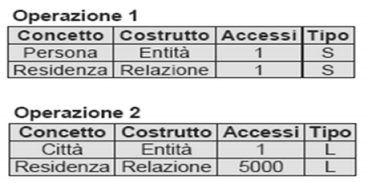
\includegraphics{images/115.PNG}
		\caption{Accessi senza ridondanza}
	\end{subfigure}
\end{figure}
\paragraph{Conclusioni} Se teniamo la ridondanza abbiamo:
\begin{itemize}
	\item Ho 1500 accessi in scrittura e 500 accessi in lettura al giorno per l'operazione 1
	\item L'operazione 2 è trascurabile.
\end{itemize}
Contando doppi gli accessi in scrittura (poichè hanno peso maggiore) otteniamo 3500 accessi al giorno. Consideriamo le stesse operazioni senza ridondanza, abbiamo:
\begin{itemize}
	\item Ho 1000 accessi in scrittura al giorno per l'operazione 1
	\item Ho 10.000 accessi in lettura al giorno per l'operazione 2
\end{itemize}
Contando doppi gli accessi (poichè hanno peso maggiore) in scrittura ho un totale di 12.000 accessi giornalieri.
\pagebreak
\subsection{Partizionamento/accorpamento di entità e relationship}
Le ristrutturazioni sono effettuate per rendere più efficienti le operazioni. Posso fare ciò \underline{riducendo gli accessi} con queste strategie
\begin{itemize}
	\item separare gli attributi di un concetto che vengono acceduti separatemente
	\item raggruppare attributi di concetti diversi acceduti insieme
\end{itemize}
Abbiamo i seguenti casi
\begin{itemize}
	\item Partizionamento di entità
	\begin{figure}[h]
		\begin{subfigure}{0.5\textwidth}
			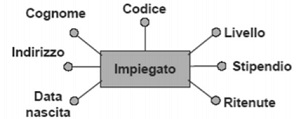
\includegraphics{images/116.PNG} 
		\end{subfigure}
		\begin{subfigure}{0.5\textwidth}
			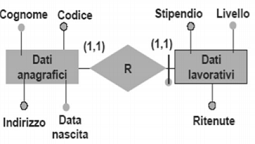
\includegraphics{images/117.PNG}
		\end{subfigure}
	\end{figure}
	\item Partizionamento di relationship
	\begin{figure}[h]
		\begin{subfigure}{0.5\textwidth}
			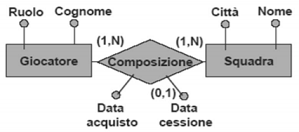
\includegraphics{images/120.PNG} 
		\end{subfigure}
		\begin{subfigure}{0.5\textwidth}
			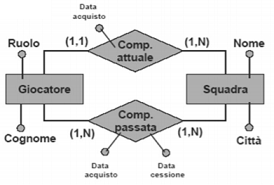
\includegraphics{images/121.PNG}
		\end{subfigure}
	\end{figure}
	\item Accorpamento di entità/relationship
	\begin{figure}[h]
		\begin{subfigure}{0.5\textwidth}
			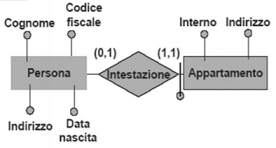
\includegraphics{images/118.PNG} 
		\end{subfigure}
		\begin{subfigure}{0.5\textwidth}
			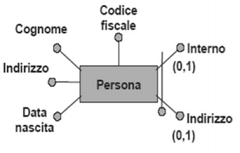
\includegraphics{images/119.PNG}
		\end{subfigure}
	\end{figure}
\end{itemize}
\paragraph{Attenzione} Valutare osservando le cardinalità!
\subsection{Traduzione verso il modello relazionale} 
In questa traduzione:
\begin{itemize}
	\item Le entità diventano relazioni sugli stessi attributi
	\item Le associazioni diventano relazioni sugli identificatori delle entità coinvolte (più gli attributi propri)
\end{itemize}
\paragraph{Relationship molti a molti} Il seguente schema
\begin{center}
	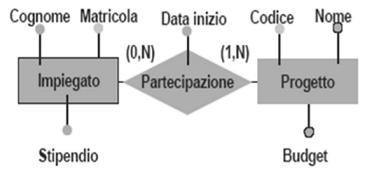
\includegraphics{images/122.PNG}
\end{center}
Mi porta ad avere le seguenti relazioni
\begin{Verbatim}[commandchars=+\[\]]
	Impiegato(+underline[Matricola], Cognome, Stipendio)
	Progetto(+underline[Codice], Nome, Budget)
	Partecipazione(+underline[Matricola, Codice], DataInizio)
\end{Verbatim}
con i seguenti vincoli di integrità referenziale:
\begin{itemize}
	\item Matricola in Partecipazione e (la chiave di) Impiegato
	\item Codice in Partecipazione e (la chiave di) Progetto
\end{itemize}
\paragraph{Nomi più espressivi per gli attributi della chiave della relazione che rappresenta la relationship} I nomi degli attributi devono rendere chiara la relazione presente. Modifichiamo la relazione Partecipazione, che diventa così (ho alterato i nomi degli attributi chiave)
\begin{Verbatim}[commandchars=+\[\]]
	Partecipazione(+underline[Impiegato, Progetto], DataInizio)
\end{Verbatim}
\paragraph{Relationship ricorsive}
\begin{center}
	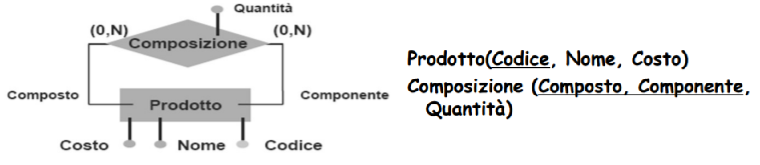
\includegraphics{images/123.PNG}
\end{center}
\paragraph{Relationship n-arie}
\begin{center}
	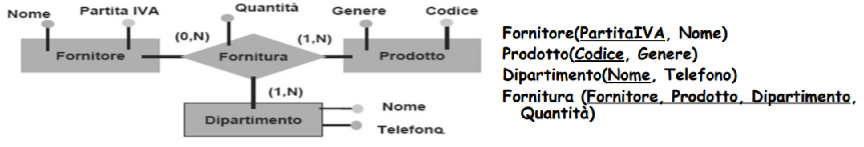
\includegraphics{images/124.PNG}
\end{center}
\pagebreak
\paragraph{Relationship uno-a-molti}
\begin{center}
	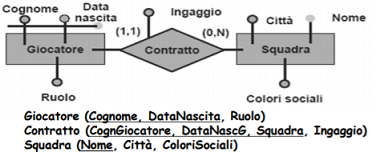
\includegraphics{images/125.PNG}
\end{center}
\paragraph{Non potrei ottenere una soluzione compatta?} Osservo che la cardinalità di Contratto rispetto a Giocatore è $(1,1)$. Posso rinunciare alla relazione Contratto ottenendo la seguente situazione
\begin{Verbatim}[commandchars=+\[\]]
	Giocatore(+underline[Cognome,DataNasc], Ruolo, Squadra, Ingaggio)
	Squadra(+underline[Nome], Città, ColoriSociali)
\end{Verbatim}
dove ho vincolo di integrità referenziale fra Squadra in giocatore e la chiave di squadra. Osservo che la cardinalità minima della relationship è 0 per Giocatore, segue che il valore dell'attributo Squadra, in Giocatore, può assumere valore nullo.
\paragraph{Entità con identificatore esterno}
\begin{center}
	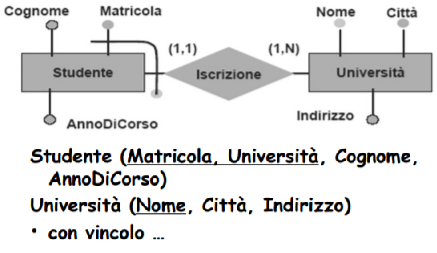
\includegraphics{images/126.PNG}
\end{center}
\paragraph{Relationship uno-a-uno} Seguono due sempi dove variano le cardinalità

\begin{figure}[h]
	\begin{subfigure}{0.5\textwidth}
		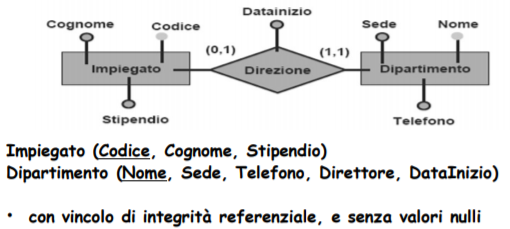
\includegraphics[width=0.9\linewidth]{images/127.PNG} 
	\end{subfigure}
	\begin{subfigure}{0.5\textwidth}
		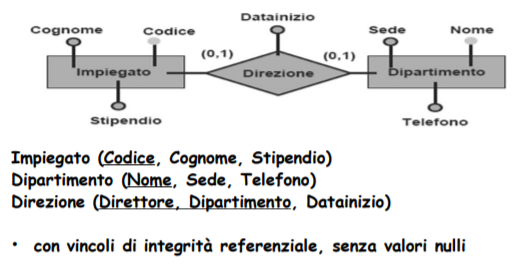
\includegraphics[width=0.9\linewidth]{images/128.PNG}
	\end{subfigure}
\end{figure}